% \documentclass[12pt,titlepage]{article}
% 
% %% THE USEPACKAGES NECESSARY FOR THIS EXAMPLE
% %% NOTE THAT genetics_manu_style MUST BE CALLED AFTER mychicago
% \usepackage{graphicx}
% %\usepackage{figcaps}
% \usepackage[nomarkers,notablist,nofiglist,tablesfirst]{endfloat}
% \usepackage{amsfonts}
% \usepackage{sectsty}
% %\usepackage{subfigure}
% %\usepackage{subcaption}
% \usepackage{natbib} \bibpunct{(}{)}{;}{author-year}{}{,} 
% \usepackage[usenames,dvipsnames,svgnames,table]{xcolor}
% %\allsectionsfont{\sffamily}
% %% THE MANUSCRIPT TITLE
% 
% \usepackage{caption}
% \usepackage[labelformat=simple]{subcaption}
% 
% \usepackage{bibentry}
% 
% \usepackage{xr}
% \externaldocument{hybrid_zone}
% 
% \newcommand{\alisa}[1]{{\em \color{red} #1}}
% \newcommand{\plr}[1]{{\em \color{blue} #1}}
% \newcommand{\yb}[1]{{\em \color{magenta} #1}}
% 
% 
% \newcommand{\given}{\,\vert\,}
% \newcommand{\st}{\,\colon\,}
% \renewcommand{\and}{\,\&\,}
% 
% 
% \begin{document}
% \setcounter{table}{0}
% \renewcommand{\thetable}{S\arabic{table}}
% \setcounter{figure}{0}
% \renewcommand{\thefigure}{S\arabic{figure}}



\begin{figure}
    \begin{center}
       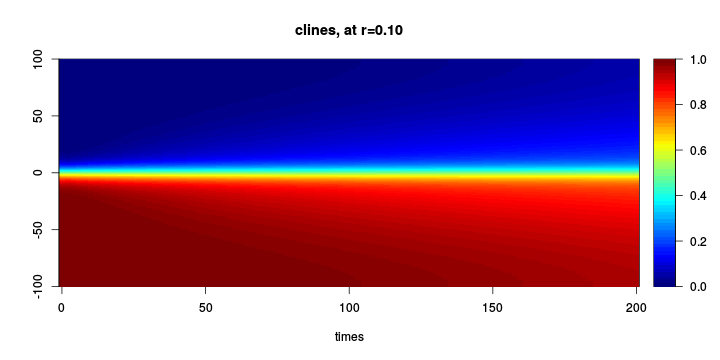
\includegraphics[width=0.7\textwidth]{figs/example_cline}
    \end{center}
    \caption{
        \textbf{Numerically computed clines,} at
        \textbf{(A)} the selected site, which forms over time $1/s$ and then remains stable, and
        \textbf{(B)} a linked site at distance $r=0.01$, which continues to smooth out as $\sqrt{t}$.
        \textbf{(C)} a linked site at $r=0.1$
        \textbf{(D)} an unlinked site.
        Other parameters.
       \plr{Do we want this figure? This one is just a placeholder; I'd put in two, that showed the formation and spread better.
       This is from the PDE (we don't have time courses from sims).}
        \label{fig:pde_clines}
    }
\end{figure}


\begin{figure}
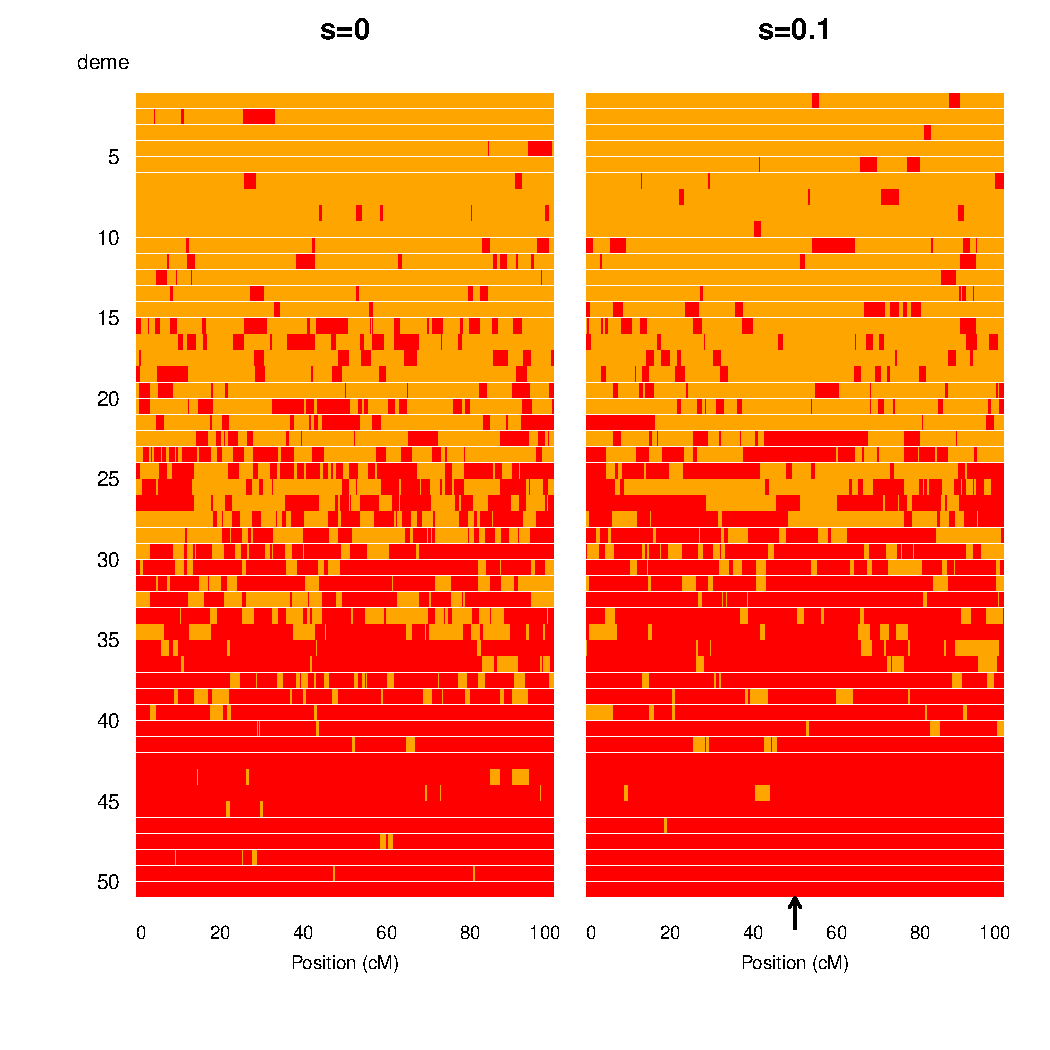
\includegraphics[width=\textwidth]{figs/plot_chromosomes_tau100}
\caption{Randomly sampled chromosomes  across a hybrid zone of age $\tau=100$. Here we compare chromosomes of length 1M from a neutral zone to one that has a single under-dominant locus ($s=0.1$) in the middle of the chromosome (indicated by black arrow). Red blocks along the chromosome denote ancestry $B$, and orange blocks are ancestry $A$. Regions surrounding the selected site are failing to introgress.
 }\label{Fig:resistanceToIntrogression100g}
\end{figure}


\begin{figure}
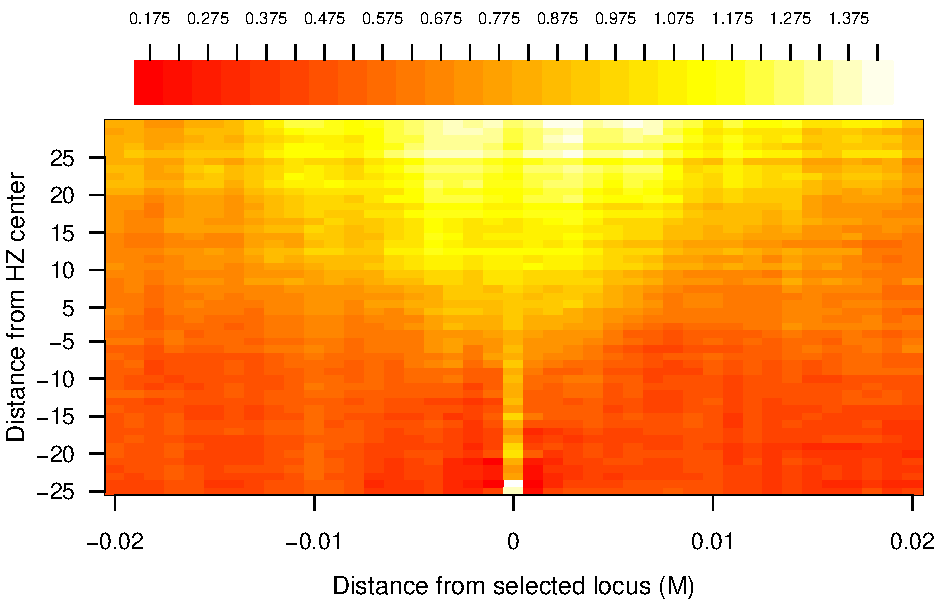
\includegraphics{figs/blocksAlongChromHeatmapAncBConditioning}
\caption{Heatmap of mean block length $l_B(m_i)$ along a simulated chromosome. }\label{Supp:blockLengthHeatmap}
\end{figure}




\begin{figure}
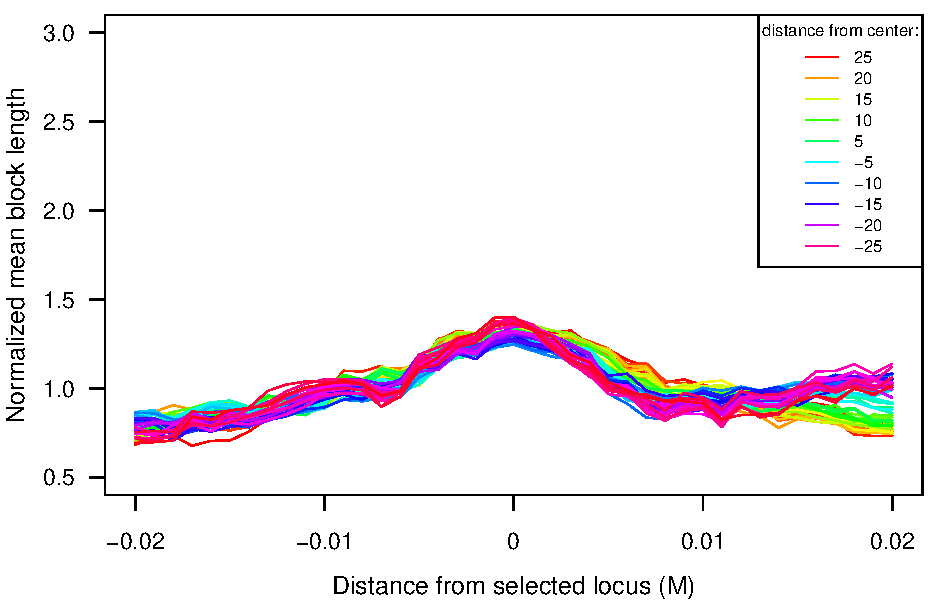
\includegraphics{figs/blocksAlongChromNoConditioning}
\caption{Heatmap of mean block length $l_\bullet(m_i)$ surrounding a given position along the genome with a single underdominant site ($s=0.01, \tau=1000$). }\label{Supp:blockLengthNoAnc}
\end{figure}

\begin{figure}
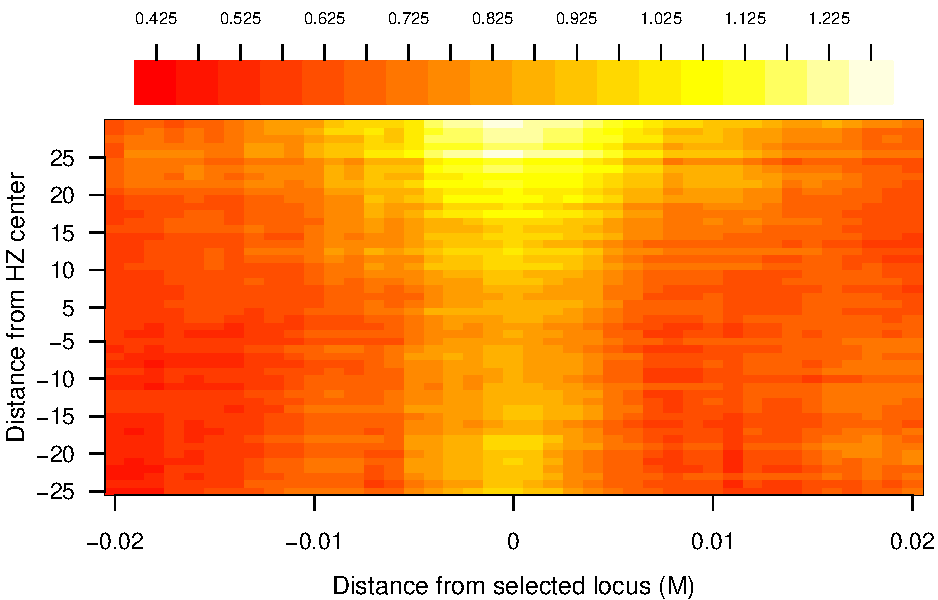
\includegraphics{figs/blocksAlongChromHeatmap}
\caption{Heatmap of mean block length $l_\bullet(m_i)$ along a simulated chromosome with a single underdominant site ($s=0.01, \tau=1000$) }\label{Supp:blockLengthHeatmapNoAnc}
\end{figure}


\begin{figure}
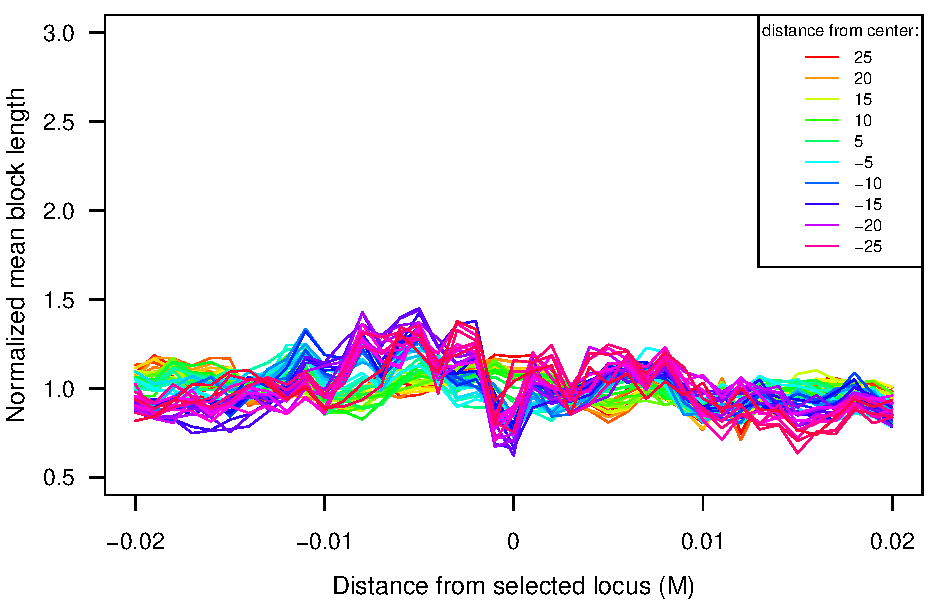
\includegraphics{figs/adjacentBlocksAlongChromAncBConditioning}
\caption{Mean block length of $l_A(m_i\cdot)$ across chromosome with single under dominant site ($s=0.01, \tau=1000$)}\label{Supp:adjacentBlocks}
\end{figure}


\begin{figure}
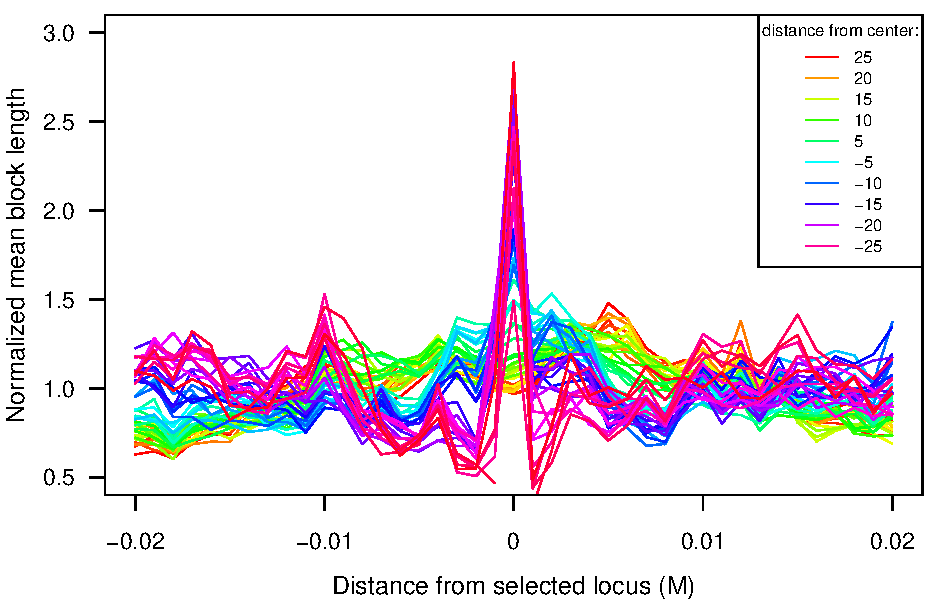
\includegraphics{figs/ratioAdjacentBlocksAlongChromAncBConditioning}
\caption{Ratio $\frac{2\sum{l_B(m_i)}}{\sum{l_A(m_i-)+I_A(m_i+)}}$ of mean block length and adjacent block lengths across a simulated chromosome with a single underdominant site ($s=0.01, \tau=1000$).  Each line represents a deme and is normalized by mean block length across the chromosome in the deme.}\label{Supp:ratioBlockAdjacent}
\end{figure}


\begin{figure}
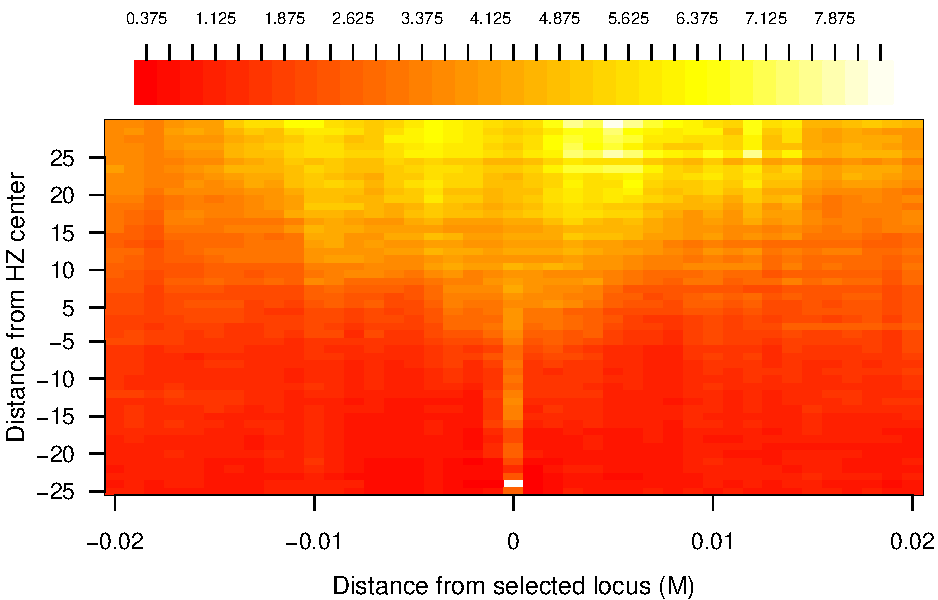
\includegraphics{figs/ratioAdjacentBlocksAlongChromHeatmapAncBConditioning}
\caption{Heatmap of $\frac{2\sum{l_B(m_i)}}{\sum{l_A(m_i-)+I_A(m_i+)}}$ across a simulated chromosome with a single underdominant site ($s=0.01, \tau=1000$). }\label{Supp:ratioBlockAdjacentHeatmap}
\end{figure}


% \end{document}
